\chapter{Specification}

\section{Legal Issues}

We used public data from twitter so direct issues of confidentiality and data-protection were avoided.

\subsection{Licensing}

We used the following software tools and packages during this project: Oracle Java, Apache Hadoop, Apache Giraph, Python, and Cytoscape. Each of these packages have permissive licences. Apache Hadoop and Giraph are licensed under the Apache licence, in accordance with this licence, a copy is included on the attached CD. Part of the project is based on last years project which is licensed according to the LGPL which is a copy-left licence, the code produced in this project is also licensed under the LGPL. A copy of this licence is also provided on the attached CD.

\subsection{Terms Of Use}

Two stipulations of the twitter API were relevant to us:

`You will not attempt or encourage others to: E) use or access the Twitter API to aggregate, 
cache (except as part of a Tweet), or store place and other geographic location information 
contained in Twitter Content.'

We don't violate this as we only store geographic information in tweets, but future extensions should be wary of it.

`Your service should not: impersonate or facilitate impersonation of others in a manner that can mislead, confuse, or deceive users.'

Again, we don't violate this but stray close enough to it in the intended use-case of our software.

https://dev.twitter.com/terms/api-terms
https://twitter.com/tos

\section{Ethical Issues}

\begin{figure}[htbp]
	\centering
	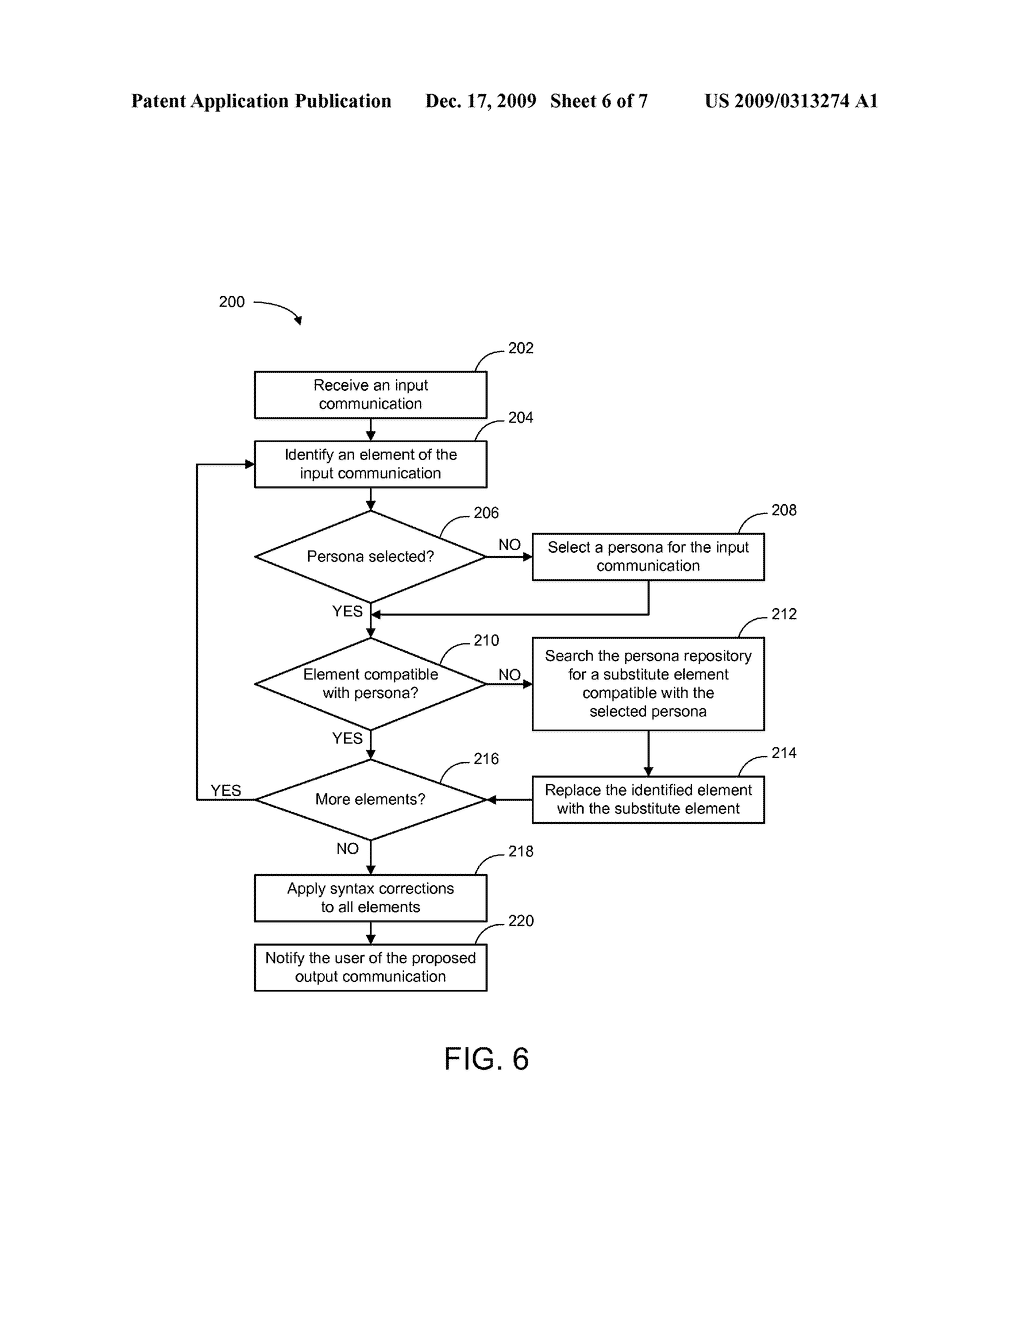
\includegraphics[width=0.7\linewidth]{img/persona_management_flow.png}
	\caption{Persona Management}
	\label{fig:persona_management_workflow}
\end{figure}

\ref{fig:persona_management_workflow}

\subsection{Surveillance}
The primary ethical issue with this project is that it is ultimately about surveillance. As someone walking a public street having no reasonable expectation of privacy doesn't quite excuse watching their every step with CCTV cameras, a user making a post on Twitter doesn't quite justify merging it into a database in an attempt to model their relationships. This issue is exacerbated by people's tendency to view posts made on public forums as being as off-the-record as a spoken conversation with a close friend.

While it could be argued that this is merely a matter of user education, what would the result of such `education' be if not stifled, warily self-conscious communications? Who wouldn't think twice about conversing with someone known to have Interesting views, and what would the effect of such isolation be on an already borderline extremist?

\subsection{Intended Use}
The application of this information may have equally chilling consequences. A simplistic view would be to claim that ultimately this is a tool that could be used for good or bad and as such the responsibility lies with the user.  In fact, the Computer Misuse Act has something to say about `dual use articles'

`In determining the likelihood of an article being used (or misused) to commit a criminal offence, prosecutors should consider the following:

    Has the article been developed primarily, deliberately and for the sole purpose of committing a CMA offence (i.e. unauthorised access to computer material)?
    Is the article available on a wide scale commercial basis and sold through legitimate channels?
    Is the article widely used for legitimate purposes?
    Does it have a substantial installation base?
    What was the context in which the article was used to commit the offence compared with its original intended purpose?'


http://www.cps.gov.uk/legal/a\_to\_c/computer\_misuse\_act\_1990/\#an10
http://www.lightbluetouchpaper.org/2007/12/31/hacking-tool-guidance-finally-appears/
http://www.guardian.co.uk/technology/2011/mar/17/us-spy-operation-social-networks

\subsection{Cracking `protected' users}
There was one boundary that we conciously decided not to cross while harvesting information from Twitter. A minority of users mark their accounts as `protected', which means that no information on their account is public. One has to send them a follow request, and then only if it is accepted will one be able to view their data. These users naturally disrupt the graph somewhat, and there are a couple of ways we could have tackled them. A fairly ethical but ineffective approach is to collate and store the information we indirectly gained on them. The alternative was to manipulate these users into accepting follow requests from our bot. Given that all our data gathering is done through a single user account, it would have been a simple matter to make the account masquerade as a member of the target group. Simply follow the most central users, and retweet the most popular tweets from those users. This would ensure that the account passed cursory examination of its `following' and tweets. This would just leave `followers' which would be easily acquired by `followbacks'; it is a common practise to follow someone who follows you, and users who follow this  practise are easily identified because they are following more people than are following them. So obtaining followers would simply be a matter of identifying these users and following them. None of this would have been a tricky addition to the existing code, but the not insignificant ethical concerns of automating impersonation on this scale prevented us.






